%-- Beamer Stuff ---
\mode<presentation>
{
  %\usetheme{umbc4}
}
\usepackage[english]{babel}
% or whatever

\usepackage[latin1]{inputenc}
% or whatever

\usepackage{times}
\usepackage[T1]{fontenc}
% Or whatever. Note that the encoding and the font should match. If T1
% does not look nice, try deleting the line with the fontenc.
%--------------------------------------------------------------------------------------------
%--- Other packages
\usepackage{pstricks}
\usepackage{pst-node}
\usepackage{pst-rel-points}

\newcommand{\change}[1]{{\red #1}}
%%%%%% Declarations Defined in custom-foils
\usebackgroundtemplate{
\includegraphics[width=\paperwidth]{oblu.eps}}%
\author[karkare]{Amey Karkare \\ \url{karkare@cse.iitk.ac.in}}
\date[IoT]{\scalebox{0.1}{\includegraphics{iitklogo.epsi}} }
\institute[CSE, IITK]{Department of CSE, IIT Kanpur}
\title[CS664]{IoT System Design}


\subtitle[IoT]{\ \\ \LARGE \psframebox[fillcolor=white,fillstyle=solid,linestyle=none]{\bf Representation of Numbers}}

\begin{document}
%%-----------------------------------------------------------------------------------------
%% New Slides
%%-----------------------------------------------------------------------------------------
\frame{\titlepage}
\usebackgroundtemplate{}

\frame{
  \frametitle{Before We Start}
  \begin{itemize}
  \item<1->{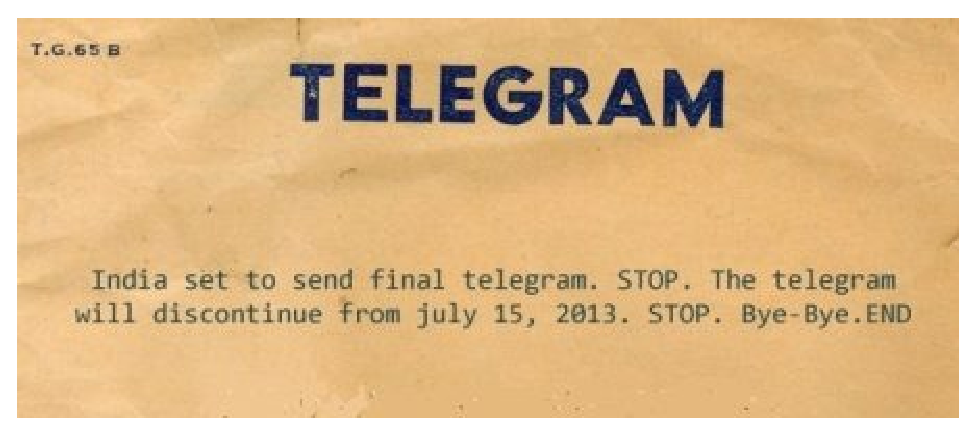
\includegraphics[width=0.5\textwidth]{Telegram.eps}\footnote{http://giglee.in/india-post/}}
  \item<2->{
\includegraphics[width=0.2\textwidth]{Twitter.eps}\footnote{\only<1>{\textcolor{white}}{https://about.twitter.com/etc/designs/about-twitter/public/img/safari-pinned-tab.svg}}}
  \item<3-> What is common to both? 
  \end{itemize}
}

\frame{
  \frametitle{Numbers}
  \begin{itemize}[<+->]
  \item There are only {\bf 10} types of people in this world
  \begin{itemize}
  \item Those who understand {\em Binary}
  \item And those who don't.
  \end{itemize}
  \item If you don't get the joke, refresh your concepts of Binary
  numbers.$_{Source\ of\ the\ joke\ not\ known.}$
  \end{itemize}
}

\frame{
  \frametitle{Binary Number System}
  \begin{itemize}[<+->]
  \item Binary system is as natural to a digital machine as
    decimal system to a man.
    \begin{itemize}[<+->]
    \item Man has 10 fingers, Learns counting using them.
    \item Digital systems have two logic states
      \begin{itemize}[<+->]
      \item 0/1 or True/False or On/Off
      \end{itemize}
    \end{itemize}
  \item A number in a number system is represented using
    digits to that system
    $$ v = d_{n-1}d_{n-2}\ldots d_2d_1d_0$$
  \item Decimal digits are 0 to 9.
  \item Binary digits are 0 and 1.
  \item Maximum value: $b^n - 1$, where $b:$ base, $n:$
    number of digits.
  \end{itemize}
}

\frame{
  \frametitle{Number System}
  \begin{itemize}[<+->]
  \item Consider the number 100011.
  \item 100011 can represent a number in any base $\geq 2$.
  \begin{itemize}[<+->]
  \item The value will be different in different bases.
  \end{itemize}
  \item When we talk about a number (say 35), we really talk
    about its value. The value of a given number is same
    irrespective of the base.
    \begin{itemize}[<+->]
    \item Confused?
    \item The confusion arises because we always have
      ``decimal'' base in mind.
    \end{itemize}
  \item  For writing it (on a paper) we need an unambiguous
    representation.
    \begin{itemize}[<+->]
    \item 'b100011 is 'h23 or 'o43 or 'd35
    \item 'o100011 is 'h8009 or 'd32777
    \end{itemize}
  \end{itemize}
}


\frame{
  \frametitle{Representation on a Computer}
  \begin{itemize}[<+->]
  \item Computers have a finite and fixed amount of storage
    for data types.
    \begin{itemize}[<+->]
    \item $n$ bit data type to contain integer can store only
      $n$ bits of information.
    \end{itemize}
  \item  Let's first consider unsigned (non-negative) numbers
    only.
    \begin{itemize}[<+->]
    \item In $n$ bits, maximum value that can be stored is
      $2^n - 1$
    \item minimum value: 0
    \end{itemize}
  \item Typical values of $n$ are powers of 2: 8, 16, 32, 64
    etc. 
  \end{itemize}
}

\frame{
  \frametitle{Signed Numbers}
  \begin{itemize}[<+->]
  \item Sign can be positive or negative.
  \item For a decimal number system, we use separate symbols
    ( ``$+$'' or ``$-$'' ) to indicate the sign. 
  \item The ``$+$'' sign is implicit most of the time.
  \item In binary system, one bit is needed for sign.
    \begin{itemize}[<+->]
    \item For example, say 0 for positive numbers, and 1 for
      negative numbers,
    \item Thus, 5 is 0101 in binary, and $-5$ is 1101.
    \end{itemize}
  \item But the story is more complex here.
  \end{itemize}
}

\frame{
  \frametitle{Signed Numbers}
  \begin{itemize}[<+->]
  \item Sign magnitude representation
    \begin{itemize}[<+->]
    \item Sign as a bit (0: positive, 1:negative)
    \item Magnitude as unsigned number 
      \begin{itemize}[<+->]
      \item in $n-1$ bits, if total $n$ bits are available.
      \end{itemize}
    \item Maximum value: $2^{n-1} - 1$, minimum value:
      $-(2^{n-1} - 1)$
    \item Two separate representation for 0: +0 and -0.
    \end{itemize}
  \item 2's complement number system
    \begin{itemize}[<+->]
    \item Easy for computations.  No separate signed
      addition/subtraction needed.
    \end{itemize}
  \end{itemize}
}

\frame{
  \frametitle{2's Complement Number System}
  \begin{itemize}[<+->]
  \item If $n$ bits are available, represent the positive
    numbers as unsigned numbers.
  \item Negative numbers are first added $2^n$, and then the
    resulting positive number is represented.
    \begin{itemize}[<+->]
    \item $2^n$ is same as 0 if only $n$ bits are used
      to represent the number.
    \end{itemize}
  \item Say n = 8. $2^n = 256$.
    \begin{itemize}[<+->]
    \item Representation of 25: 00011001
    \item Representation of $-25 \equiv$ Representation of
      $231 (256 - 25): 11100111$
    \end{itemize}
  \item Max value: $2^{n-1} - 1$. Min value: $-2^{n-1}$.
    \begin{itemize}[<+->]
    \item Proof: Practice Exercise.
    \end{itemize}
  \end{itemize}
}

\frame{
  \noindent\pnode(0.5\textwidth,-0.1\textheight){pos}
  \rput(pos){\special{ps: 0.9 .setopacityalpha}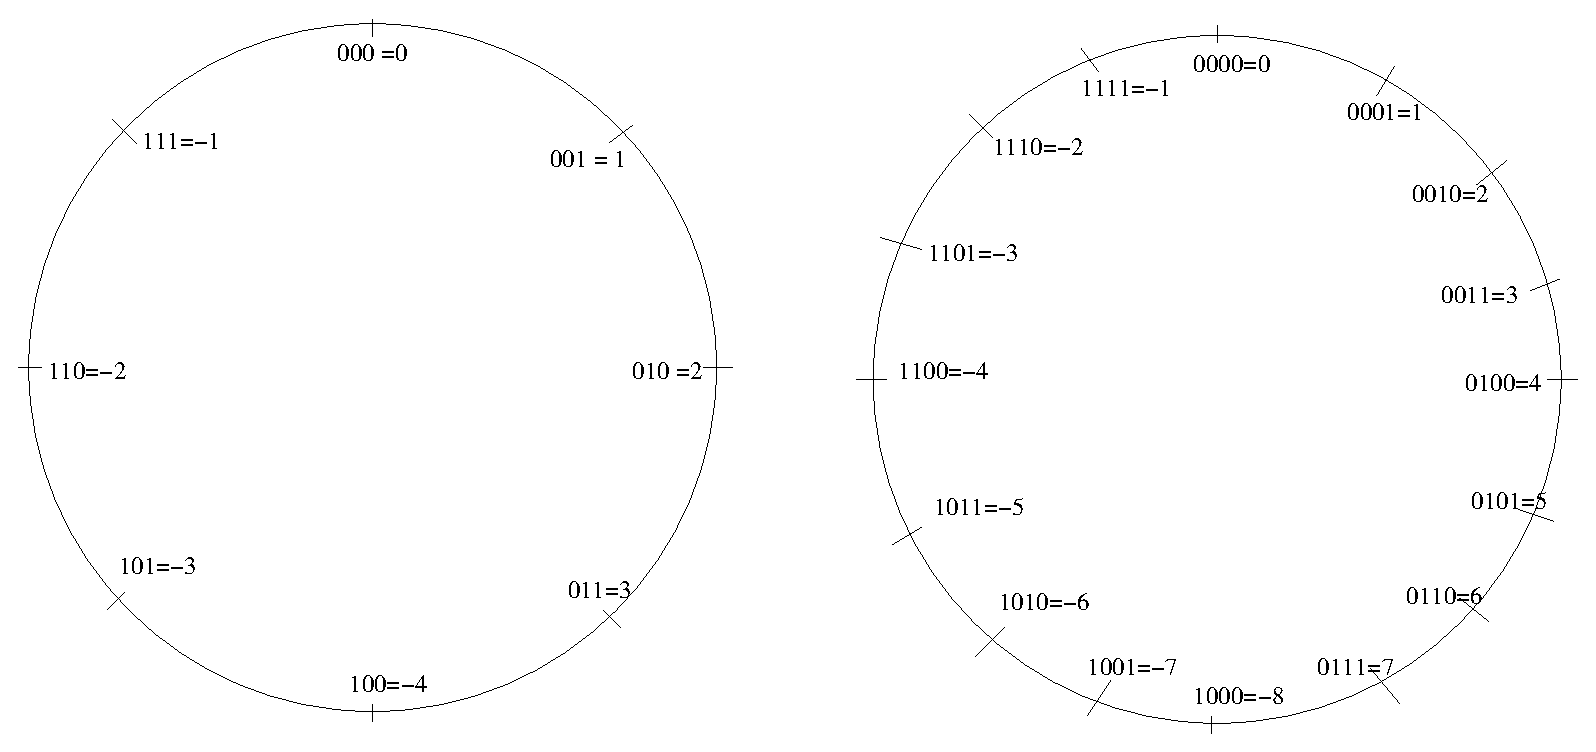
\includegraphics[width=0.8\textwidth]{NumberCircle.eps}}

  %  \begin{center}
  %    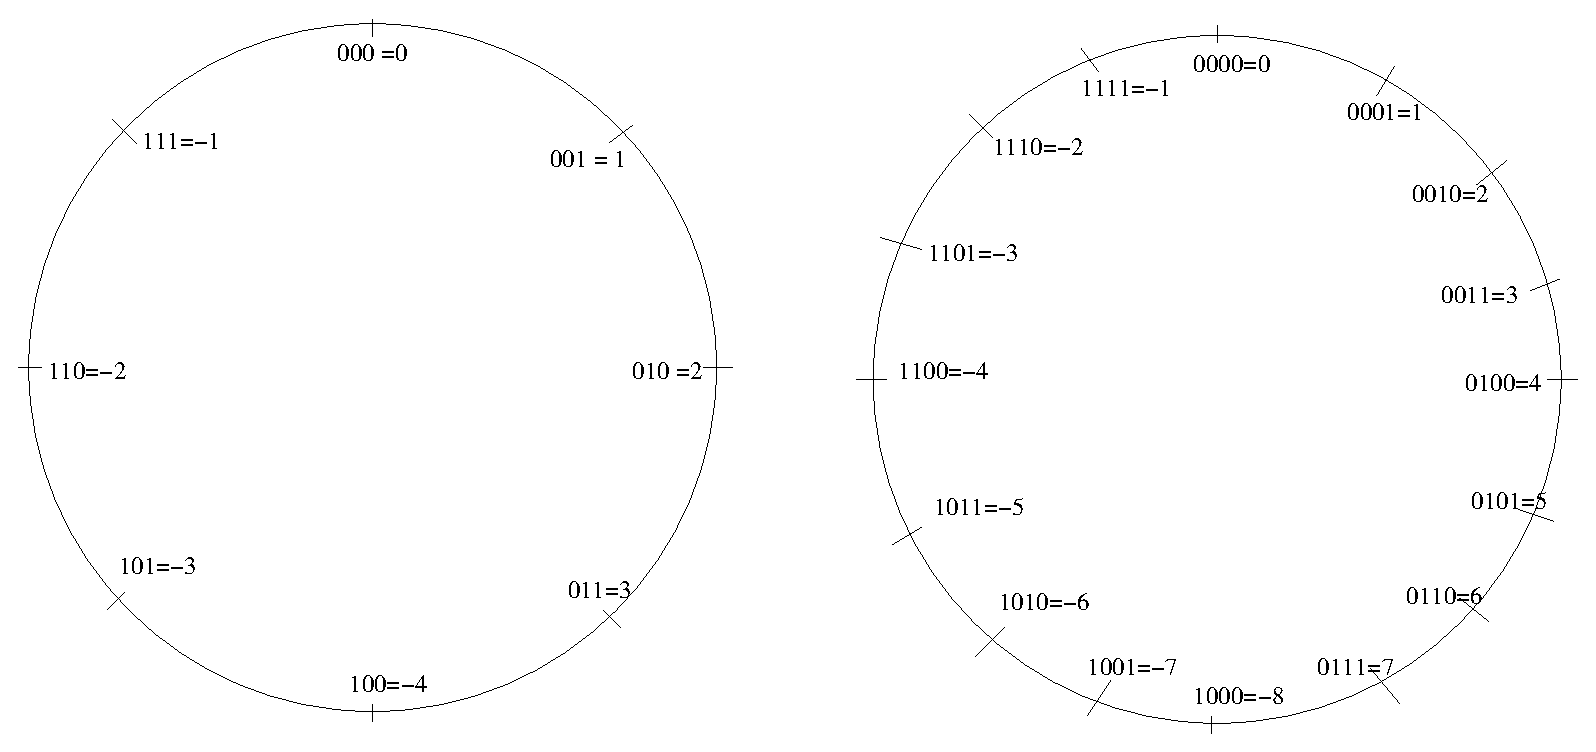
\includegraphics[width=.8\textwidth]{NumberCircle.eps}
  %  \end{center}
  \frametitle{2's Complement Numbers}
  \rule{0pt}{3cm}
  \begin{itemize}[<+->]
  \item Signed numbers in $3$-bit and $4$-bit
    representation
  \item What is the relationship between
    \begin{itemize}[<+->]
    \item $+2$ in $3$-bits and $+2$ in $4$-bits?
    \item $-2$ in $3$-bits and $-2$ in $4$-bits?
    \end{itemize}
  \item Does this hold for other numbers as well?
    \begin{itemize}[<+->]
    \item Sign extension : $0$ for positive numbers, $1$ for
      negative numbers. 
    \item Proof: Practice Exercise.
    \end{itemize}
  \end{itemize}
}

\frame{
  \frametitle{2's Complement Numbers}
  \begin{itemize}[<+->]
  \item To compute representation of a negative number
    faster,
    \begin{itemize}[<+->]
    \item find the representation of its absolute value in
      $n$ bits.
    \item invert all bits of this number and add 1 to it.
    \end{itemize}
  \item For example, $-10$ in $8$ bits
    \begin{itemize}[<+->]
    \item 10 in 8 bits is 00001010.
    \item Invert all bits to get: 11110101.
    \item Add 1 to it to get: 11110110.
    \end{itemize}
  \end{itemize}
}

\frame{
  \frametitle{2's Complement Makes Arithmetic Easy}
  \begin{itemize}[<+->]
  \item For addition $A + B$, Add bit patterns of two numbers
    irrespective of whether the numbers are positive or
    negative.
  \item For subtraction $A - B$, use addition of $A + (-B)$.
    $-B$ can be found by 2's complement.
  \item Booth's Multiplication
  \end{itemize}
}

\newcommand{\xor}{
  \psset{unit=1mm}
  \begin{pspicture}(0,0)(5,12)
    %%\psframe(-3,-5)(5,12)
    \psparabola(5,6)(1,0)
    \psparabola(5,6)(1,5)
    \psparabola(5,7)(1,6)
    \psline(-1,5)(-1,13) %in-left
    \psline(3,5)(3,10)   %in-right
    \psline(1,0)(1,-4.5)   %out
  \end{pspicture}
}

\frame{
  \frametitle{Adder and Subtractor}
  \begin{center}
    \psset{unit=1mm}
  \begin{pspicture}(-10,-10)(70, 45)
    %%\psgrid[unit=10mm](0,0)(70mm, 45mm)
    %%\psframe(-10,-10)(70, 45)
    %% INPUT B
    \alt<2>{
    \putnode{x0}{origin}{9}{30}{\xor}
    \putnode{x1}{x0}    {9}{ 0}{\xor}
    \putnode{x2}{x1}    {9}{ 0}{\xor}
    \putnode{x3}{x2}    {9}{ 0}{\xor}
    }{
    \psline(9, 36)(9,19.5)
    \psline(12, 36)(12,19.5)
    \psline(15, 36)(15,19.5)
    \psline(18, 36)(18,19.5)
    }
    %% Adder itself
    \putnode{a0}{origin}{30}{13}{
      \psframebox[framesep=5]{$\qquad\qquad$ADDER$\qquad\qquad$}}
    %% INPUT A
    \psline(45, 36)(45,19.5)
    \psline(48, 36)(48,19.5)
    \psline(51, 36)(51,19.5)
    \psline(54, 36)(54,19.5)

    %% OUTPUT
    \psline(25, 6.5)(25,-4)
    \psline(28, 6.5)(28,-4)
    \psline(31, 6.5)(31,-4)
    \psline(34, 6.5)(34,-4)

    %% Cin and Cout
    \psline(58,13.5)(65,13.5)
    \rput(-1,11){{\footnotesize C\_in}}
    \psline(-4,13.5)(3,13.5)
    \rput(64,11){{\footnotesize C\_out}}
    %%Add/sub
    \alt<2>{
    \psline(-8,34)(36.7,34)
    \rput(-9,36){{\footnotesize Subtract (1)}}
    \rput(-6,39){{\footnotesize Add (0) /}}
    \psline(-4,34)(-4,13.5)
    }{}
    \alt<2>{
    \putnode{inpB}{a0}{-10}{27}{$\stackrel{B}{\overbrace{\rule{36mm}{0pt}}}$}
    }{
    \putnode{inpB}{a0}{-10}{27}{$\stackrel{B}{\overbrace{\rule{12mm}{0pt}}}$
      \rule{12mm}{0pt}}
    }
    \putnode{inpA}{inpB}{29}{0}{$\stackrel{A}{\overbrace{\rule{12mm}{0pt}}}$}
  \end{pspicture}
  \end{center}
}


\frame {
  \frametitle{Real Numbers}
  \begin{itemize}[<+->]
  \item All real numbers can not be represented in computers
    \begin{itemize}[<+->]
    \item By definition, between any two distinct real
      numbers, there are infinite number of real numbers.
    \end{itemize}
  \item First we need to understand the binary representation
    of real numbers.
  \end{itemize}
}

\frame{
  \frametitle{Real Numbers}
  \begin{center}{\small
      \rnode{D1}{Binary Point} \rule{50mm}{0mm} \\ [3mm]
      \psframebox{\rnode{I0}{1110}\rnode{D0}{ $\bullet$ }\rnode{F0}{1101}}
      \ \ Value = $2^3 + 2^2 + 2^1 + 2^{-1} + 2^{-2} + 2^{-4} = 14.8125$ \\ [3mm]
    \rnode{I1}{Integral Part}\ \ \ \ \ \ \ \
    \rnode{F1}{Fractional Part}\rule{50mm}{0mm}
    \nccurve[angleA=-90, angleB=90, nodesepB=.1]{->}{D1}{D0}
    \nccurve[angleA=90, angleB=-90, nodesepB=.1]{->}{I1}{I0}
    \nccurve[angleA=90, angleB=-90, nodesepB=.1]{->}{F1}{F0}
  }\end{center}
  \begin{itemize}[<+->]
  \item Binary point is analogous to the decimal point.
  \item It differentiates between binary integral part and
    binary fractional part.
    \begin{itemize}[<+->]
    \item Decimal point differentiates between decimal
      integral part and decimal fractional part.
    \end{itemize}
  \item   Positional value of each binary digit 
    \begin{itemize}[<+->]
    \item $2^i$ for the integral part 
    \item $1/2^i$ for the fractional part 
    \end{itemize}
  \end{itemize}
}

\frame{
  \frametitle{Real Numbers: Fixed Point}
  \begin{itemize}[<+->]
  \item Assume that we have $n$ bits to represent a real
    number.
  \item If the position of binary point is fixed (say 4
    locations from the right)
    \begin{itemize}[<+->]
    \item We do not need to store any information about the
      binary point.
    \end{itemize}
  \item Bit pattern $11101101$ is 8-bit fixed point
    representation with implied binary point at fourth bit
    from the right (1110.1101).
    \begin{itemize}[<+->]
    \item This bit pattern is for 14.8125 in decimal.
    \item Same bit pattern, when treated as unsigned number, 
      indicates 237.
    \end{itemize}
  \item In general a bit pattern for a fixed point number $f$
    is same as the bit pattern for number $f \times 2^i$,
    where $i$ is the position of implied binary point.
    \begin{itemize}[<+->]
    \item Fixed point numbers can be signed or unsigned.
    \end{itemize}
  \item Precision : $2^{-i}$
  \item Range: $2^{-i}$ times the range of the corresponding integer.
  \end{itemize}
}

\frame{
  \frametitle{Fixed Point Numbers}
  \begin{itemize}[<+->]
  \item Advantage:
    \begin{itemize}[<+->]
    \item Simple format: Same as integer format
    \item Simple algorithms: 
      \begin{itemize}[<+->]
      \item Add/Subtract: Same as integer add/subtract
      \item Multiply/Divide: Integer multiply/divide followed
        by bit shift
      \end{itemize}
    \end{itemize}
  \item Disadvantage:
    \begin{itemize}[<+->]
    \item If the data set is large, one ends up having huge
      size of data structure.
      \begin{itemize}[<+->]
      \item For example, if a variable is needed to be able
        to store mass of a planet or mass of a person to
        reasonable accuracy, it will have large number of
        bits for the integer part.
      \end{itemize}
    \end{itemize}
  \end{itemize}
}

\frame{
  \frametitle{Scientific Representation}
  \begin{itemize}[<+->]
  \item Numbers in scientific representation are stored with
    significand and exponent.
    \begin{itemize}[<+->]
    \item Mass of an electron: $9.1 \times 10^{-28} g$
    \item Mass of a person: $6.0 \times 10^4 g$
    \end{itemize}
  \item In standard (normalized) form, significand is between
    $[1.0, 10)$.
  \item Zero can not be written as a number in normalized form.
  \end{itemize}
}

\frame{
  \frametitle{Scientific Numbers in Binary}
  \begin{itemize}[<+->]
  \item Exponents are powers of $2$.
  \item Significands are binary.
  \item In normalized form, significand is between $[1.0,
    2)$.
    \begin{itemize}[<+->]
    \item Integer part is always $1.xxxx$
    \end{itemize}
  \item $1.0011E100$ represents \pause $1.0011 \times
    2^{100}$ \pause or
    'b$10011$ or $19$.
  \end{itemize}
}

\frame{
  \frametitle{Floating Point Numbers}
  \begin{itemize}[<+->]
  \item Exponents can be positive or negative.
    \begin{itemize}[<+->]
    \item Exponents are stored as biased integers.
      \begin{itemize}[<+->]
      \item If $e$ is the exponent, then $e+b$ is stored as
        unsigned number for exponent.
      \item $b$ is the bias.
      \end{itemize}
    \end{itemize}
  \item Numbers are normalized.
    \begin{itemize}[<+->]
    \item Significand is of the form $1.xxxx\ldots$
    \item ``$1.$'' need not be stored!
    \end{itemize}
  \end{itemize}
}

\frame{
  \frametitle{IEEE754 Single Precision Numbers}
  \begin{itemize}[<+->]
  \item Used by most programming languages as {\bf float}
    data type.
  \item 32 bit wide
  \item Includes
    \begin{itemize}[<+->]
    \item Sign: Sign of the number
    \item Mantissa: Significand without leading ``1.0''
    \item Exponent: biased by 127 or excess-127.
    \end{itemize}
  \end{itemize}
}

\frame{
  \frametitle{IEEE754 Single Precision Numbers}
  \begin{center}
  \begin{tabular}{c|@{}lr@{}|@{}lr@{}}
    31&30&23&22&0 \\ \hline
    \multicolumn{1}{|c|}{S} &
    \multicolumn{2}{|c|}{
      \begin{tabular}{c}
        Exp \\ excess-127
      \end{tabular}
    } &
    \multicolumn{2}{|c|}{\rule{20mm}{0pt} Mantissa \rule{20mm}{0pt}} \\ \hline
  \end{tabular}
  \end{center}
  Consider $-24.75$ in decimal \\ [2mm] \pause
  \begin{tabular}{ll}
    In Binary:& $-11000.11$\\\pause
    Scientific Binary:& $-1.100011 \times 2^4$ \\\pause
    Sign:& $1$ (Negative) \\\pause
    Exponent:& $4+127 = 131$ or $10000011$ in binary \\\pause
    Mantissa:& $100011000000000000000000$ \\\ \\\pause
    IEEE754 Bit pattern:&
    $1\ 10000011\ 100011000000000000000000$ \\
    In Hex:& 'hC1C60000
  \end{tabular}
}

\frame{
  \frametitle{Double Precision Numbers}
  \begin{itemize}[<+->]
  \item 64 Bits in size.
    \begin{itemize}[<+->]
    \item Sign: 1 bit
    \item Exponent: 11 bit excess-1023
    \item Mantissa: 52 bits
    \end{itemize}
  \end{itemize}
}

\frame{
  \frametitle{Problems with Representation}
  \pause
  \begin{itemize}[<+->]
  \item Can not represent $0.0$ in this way.
    \begin{itemize}[<+->]
    \item There is no ``$1.$'' prefix in its representation. 
    \end{itemize}
  \item Real number computations also need $\pm\infty$.
  \end{itemize}
}

\frame{
  \frametitle{Special Cases}
  \begin{itemize}[<+->]
  \item $+0.0$ or $-0.0$:
    \begin{itemize}[<+->]
    \item Sign: $0$ (for $+$), $1$ (for $-$).
    \item Exponent and Mantissa: all zeroes.
    \end{itemize}
  \item Bit pattern for an integer $0$ is same as bit pattern
    for float $+0.0$.
  \item $\pm\infty$:
    \begin{itemize}[<+->]
    \item Sign: $0$ (for $+$), $1$ (for $-$).
    \item Exponent: All $1$s (0xFF for single precision,
      0x7FF for double precision).
    \item Mantissa: All zeroes.
    \end{itemize}
  \end{itemize}
}

\frame{
  \frametitle{Special Cases}
  \begin{itemize}[<+->]
  \item Not-a-Number (NaN)
    \begin{itemize}[<+->]
    \item Exponent: All $1$s.
    \item Mantissa: Other than all zeroes.
    \end{itemize}
  \item Denormalized numbers:
    \begin{itemize}[<+->]
    \item Needed to store small intermediate results.
    \item Exponent: All zeroes.
    \item Mantissa: Other than all zeroes.
    \item Assumed to be as: $0.m \times 2^{1-b}$.
    \end{itemize}
  \end{itemize}
}

\frame{
  \frametitle{Limits}
  \begin{itemize}[<+->]
  \item Max normalized value:
    \begin{itemize}[<+->]
    \item Exponent: 0xFE (single precision, SP) or 0x7FE
      (double precision, DP)
      \begin{itemize}[<+->]
      \item Or $2^{127}$ (SP), $2^{1023}$ (DP)
      \end{itemize}
    \item Mantissa: $111\ldots111$
      \begin{itemize}[<+->]
      \item Significand: Close to $2$ with assumed ``$1.$''
        prefix.
      \end{itemize}
    \item Max value of $\approx 2^{128}$ (SP), $\approx
      2^{1024}$ (DP)
    \end{itemize}
  \item Min positive normalized value:
    \begin{itemize}[<+->]
    \item Exponent: 0x01 $\Rightarrow$ $2^{-126}$(SP),
      $2^{-1022}$ (DP)
    \item Mantissa: $000\ldots000$ or $1.0$
    \item Min value: $2^{-126}$(SP),
      $2^{-1022}$ (DP)
    \end{itemize}
  \item Precision: $2^{e-23}$ (SP), $2^{e-52}$ (DP)
    \begin{itemize}[<+->]
    \item Precision is relative to the number (exponent = $e$)
    \end{itemize}
  \end{itemize}
}

\frame{
  \frametitle{Limits for Denormalized Numbers}
  \begin{itemize}[<+->]
  \item Min (positive) value:
    \begin{itemize}[<+->]
    \item Mantissa: $000\ldots 001$
    \item Exponent: $000\ldots 000$
    \item $2^{-149}$ for SP, $2^{-1074}$ for DP
    \end{itemize}
  \item Max (positive) value:
    \begin{itemize}[<+->]
    \item Mantissa: $111\ldots 111$ ($\equiv 0.111\ldots 111
      \approx 1.0$)
    \item Exponent: $000\ldots 000$
    \item $\approx 2^{-126}$ (SP), $\approx 2^{-1022}$ (DP)
    \end{itemize}
  \end{itemize}
}
\end{document}
